\documentclass{beamer}
\usepackage{lipsum}
\usepackage[brazilian]{babel}
\usepackage[utf8]{inputenc}

\usepackage{enumerate}
\usepackage{dcolumn}
\usepackage{tabu}
\usepackage{colortbl}
\usepackage{booktabs}
\usepackage{changes}
\usepackage{listings}
\usepackage{placeins}
\usepackage{amsmath}

\usepackage{multirow}

\newcommand*{\Scale}[2][4]{\scalebox{#1}{$#2$}}%
\newcommand*{\Resize}[2]{\resizebox{#1}{!}{$#2$}}%

\usetheme[faculty=ppca,language=logo,framenumber,totalframenumber]{UniversiteitGent}

\title{Implantando o barramento de serviços ERLANGMS no CPD/UFSM}
\subtitle{ \textcolor{black}{Universidade Federal de Santa Maria} \\
			\textcolor{black}{\small{Centro de Processamento de Dados}} 
}



\author{Everton de Vargas Agilar (UnB / UFSM) \\
		Jader Adiel (UFSM)
}



\begin{document}

\begin{frame}
  \titlepage
\end{frame}




%%##################### PLANO #########################################

\section{Plano}


\subsection{Plano}

\begin{frame}
  \frametitle{Plano}

    \begin{itemize}

	    \item<1-> Barramento de Serviços ERLANGMS
		    \begin{itemize}
		  	  \item<1->Contexto e justificativa do projeto
	    	  \item<1->Histórico do projeto
	    	  \item<1->Envolvimento e organização da equipe de desenvolvimento
  	  	 	  \item<1->Funcionalidades implementadas e em uso na UnB
  	  	 	  \item<1->Design da arquitetura
		    \end{itemize}
	   	  \item<1-> 

	    \item<1-> Implantação do barramento na UFSM
		    \begin{itemize}
			\item<1->Modernização do SIE
			    \begin{itemize}
					\item<1->Expectativas e viabilidade
					\item<1->Desafios da migração do backend Delphi para Java
					\item<1->Plano de desenvolvimento da versão 2.0
				\end{itemize}
			\item<1->Caso prático 1: Web services implementados para o NCC
			\item<1->Caso prático 2: TClis do SIE invocando web services Java
		    \end{itemize}
   	    \item<1-> 
   	    


	 \end{itemize}	   	  

\end{frame}




%%##############################################################




\section{Barramento de Serviços ERLANGMS}


\subsection{Contexto e justificativa do projeto}


\begin{frame}
  \frametitle{Contexto}

  \begin{exampleblock}{Modernização de Sistemas Legados}
  
  “\textbf{Legacy information systems} are typically the
	backbone of an organization’s information flow
	and the main vehicle for consolidating business
	information. They are thus mission critical, and
	their failure can have a serious impact on
	business.” [BENNET95]

	\vspace{0.5cm} 

	“Migrate Systems Incrementally recommends that the old system be
	gradually and incrementally replaced by the new system. New
	results can then be integrated as you proceed...” [DEMEYER et al. 2002]
  \end{exampleblock}

  
\end{frame}




%%##############################################################



\begin{frame}
  \frametitle{Objetivos}
  
    \begin{itemize}
       \item<1-> Propor uma abordagem para modernizar os sistemas legados de
forma orientada a serviços (SOA) composto por:

    \begin{itemize}
       \item<1->um barramento de serviços;
       \item<1->um processo de modernização para guiar os trabalhos de modernização de software; 
       \item<1->um kit de desenvolvimento (SDK) para implementar serviços independente da
       linguagem de programação.
    \end{itemize}
				
    \end{itemize}
    
\end{frame}





\begin{frame}
  \frametitle{Justificativa}
  
    \begin{itemize}
       \item<1->Maximizar o reuso dos fluxos de negócios;
       \item<1->Modernizar os sistemas de maneira sistemática e incremental;
       \item<1->Minimizar dependências tecnológicas; 
       \item<1->Experimentar SOA (Service Oriented Architecture).
    \end{itemize}
    
\end{frame}


\subsection{Panorama geral sobre modernização na literatura}


\begin{frame}
  \frametitle{Justificativa \\ \small{Panorama geral sobre modernização na literatura}}

 	%% Mostra o diagrama de bolhas
  	
	\begin{figure}
	\centering
		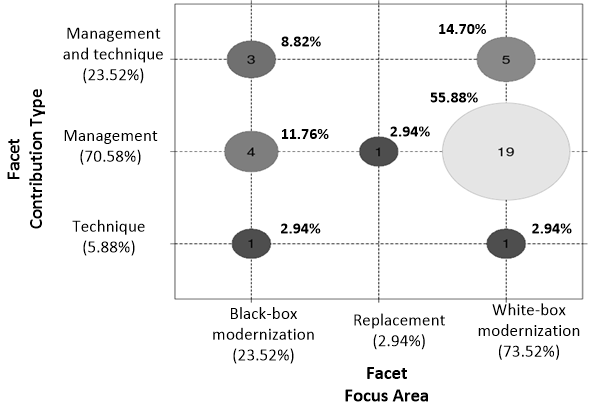
\includegraphics[scale=0.45]{img/bubble_diagram.png}
	\end{figure}
  
\end{frame}



%%##############################################################


\section{Plataforma agnóstica de serviços}


\begin{frame}[c]{ }
\centering
  \huge{Plataforma agnóstica de serviços}
\end{frame}



\subsection{Sobre}


\begin{frame}
  \frametitle{Plataforma agnóstica de serviços}

  \begin{exampleblock}{ERLANGMS}
  
É uma plataforma de software desenvolvida para facilitar a integração de sistemas por meio de um barramento 
de serviços multiplataforma orientado a contratos de serviços + SDK + Processo de modernização e arquitetura documentado (SMSOC).

  \end{exampleblock}

  
\end{frame}


\begin{frame}
  \frametitle{Plataforma agnóstica de serviços}

  \begin{exampleblock}{Características do barramento}
  
	  \begin{itemize}
		\item<1->Multiplataforma e arquitetura modular;
	    \item<1->Serviços especificados em catálogos de serviços;
	    \item<1->Cluster de serviços (Ex.: Erlang nodes, JBoss Containers) para evitar ponto único de falhas;
    	    \item<1->Suporta serviços RESTful;
   	    \item<1->Modelo de concorrência: Actor Model;
    	    \item<1->Fácil compilação e instalação.
	  \end{itemize}

  \end{exampleblock}

  
\end{frame}


\begin{frame}
  \frametitle{Plataforma agnóstica de serviços}

  \begin{exampleblock}{Principais recursos/features}
  
	  \begin{itemize}
		\item<1->HTTP/2, HTTP/1.1, HTTPS (Secure TLS Listener);
	    \item<1->LDAP v3 -- Proxy LDAP;
	    \item<1->HTTP Basic authentication;
    	    \item<1->OAuth2 authentication (em progresso);
		\item<1->SDK para criar serviços em Java e .Net (suspenso);
		\item<1->Api query -- filter, fields, sort, limit.
	  \end{itemize}

  \end{exampleblock}

  
\end{frame}


\begin{frame}
  \frametitle{Plataforma agnóstica de serviços}

  \begin{exampleblock}{Principais recursos/features experimentais}
  
	  \begin{itemize}
 	    \item<1->Suporte para Dados Abertos;
    	    \item<1->JSON Schema Draft 4 para descrever/validar a entrada/saída no payload das mensagens REST;
	    \item<1->Django template (processamento de template no back-end).
	  \end{itemize}

  \end{exampleblock}

  
\end{frame}




%%##############################################################



\section{Principais Resultados do Trabalho}


\begin{frame}[c]{ }
\centering
  \huge{Principais Resultados do Trabalho}
\end{frame}



\begin{frame}
  \frametitle{Desenvolvimento de serviços com o SDK}

	\begin{figure}
	\centering
		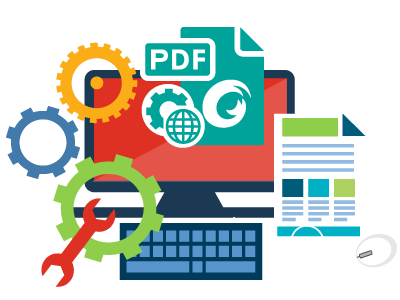
\includegraphics[scale=0.4]{img/sdk.png}
	\end{figure}
  
\end{frame}


\begin{frame}
  \frametitle{Autenticação de usuários com o proxy LDAP}

	\begin{figure}
	\centering
		
\includegraphics[scale=0.6]{img/ldap.png}
	\end{figure}
  
\end{frame}


\begin{frame}
  \frametitle{Autenticação e autorização de serviços REST com OAuth2}

	\begin{figure}
	\centering
		
\includegraphics[scale=0.4]{img/oauth2.png}
	\end{figure}
  
\end{frame}



\begin{frame}
  \frametitle{Trabalhos futuros}

  \begin{exampleblock}{Trabalhos futuros}
  
	  \begin{itemize}
 	    \item<1->Portal Api Management;
    	    \item<1->JSON Schema Draft 4;
    	    \item<1->SDK .Net.
	  \end{itemize}

  \end{exampleblock}

  
\end{frame}


%%##############################################################


\subsection{Perguntas}


\begin{frame}[c]{ }
\centering
  \huge{Perguntas ?}
\end{frame}


\begin{frame}
  \frametitle{Perguntas}

  \begin{exampleblock}{}
  
	  \begin{itemize}
		\item<1->(QP1) Por que Erlang/OTP?
		\item<1->(QP2) Quem usa Erlang/OTP?
	    \item<1->(QP3) Por que o desenvolvimento de um novo barramento em vez de utilizar um existente?
	    \item<1->(QP4) Por que não implementar web services usando somente Java e seus frameworks?
	  \end{itemize}
  
  \end{exampleblock}

  
\end{frame}


\begin{frame}
  \frametitle{(QP1) Por que Erlang/OTP?}

    \begin{itemize}
       \item<1-> Suporta aplicações distribuídas e tolerantes a falhas a serem executadas em um ambiente de tempo real e ininterrupto;
       \item<1-> Possui um ambiente de execução que realmente facilita o desenvolvimento de software de rede e de clusters de serviços;
       
       \item<1-> Possui um modelo de arquitetura baseado em atores (Actor Model) onde os processos podem 
       se comunicar apenas por mensagens.
       
    \end{itemize}
  
\end{frame}


\begin{frame}
  \frametitle{(QP2) Quem usa Erlang/OTP?}

	  \begin{itemize}
		\item<1->Facebook (Backend do chat -- 100 milhões de usuários ativos);
		\item<1->Whatapps (Servidores de mensagens -- 2 milhões de usuários/servidor);
		\item<1->Yahoo (Delicious -- 5 milhões de usuários e mais de 150 milhões de bookmarks);
		\item<1->Amazon SimpleDB, o serviço de dados do Amazon EC2;
		\item<1->GitHub (Backend -- milhares de transações concorrentes);
		\item<1->T-Mobile nos seus sistemas de SMS e autenticação;
		\item<1->Motorola, CouchDB, RabbitMQ, Ejabbed, entre outros.
						
	   \end{itemize}
  
\end{frame}


\begin{frame}
  \frametitle{(QP3) Por que um novo barramento?}

	  \begin{itemize}
		\item<1->Obter domínio sobre as tecnologias e o design RESTful;
		\item<1->Barramento de serviços são produtos caros e complexos;
		\item<1->Disponibilizar um produto simples (contém somente 10 mil linhas de código atualmente).
					
	   \end{itemize}
  
\end{frame}


\begin{frame}
  \frametitle{(QP4) Por que não implementar web services em Java com frameworks?}

	  \begin{itemize}
		\item<1->É uma opção, mas exige ferramentas para gerenciar;
		\item<1->Não é orientado a contrato de serviços;
		\item<1->Não é independente de linguagem de programação;
		\item<1->Não é escalável apenas usando os frameworks.
	   \end{itemize}
  
\end{frame}



\begin{frame}[c]{ }
\centering
  \huge{Obrigado!}
\end{frame}


\end{document}



